\documentclass[tikz, convert = false]{standalone}%

\usepackage[utf8]{inputenx}%  http://ctan.org/pkg/inputenx
% Euler for math | Palatino for rm | Helvetica for ss | Courier for tt
\renewcommand{\rmdefault}{ppl}% rm
\linespread{1.05}% Palatino needs more leading
\usepackage[scaled]{helvet}% ss //  http://ctan.org/pkg/helvet
\usepackage{courier}% tt // http://ctan.org/pkg/courier
\usepackage{eulervm}  %  http://ctan.org/pkg/eulervm
% a better implementation of the euler package (not in gwTeX)
\normalfont%
\usepackage[T1]{fontenc}%  http://ctan.org/pkg/fontenc
\usepackage{textcomp}%  http://ctan.org/pkg/textcomp

\usetikzlibrary{intersections}
\usetikzlibrary{calc}

\begin{document}
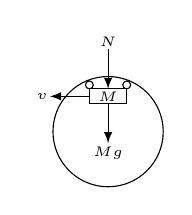
\begin{tikzpicture}
  \coordinate (O) at (0, 0);
  \draw[name path = circ] (O) circle[radius = 0.7];

  \path[name path = line] (-0.7, 0.65) -- +(1.4, 0);
  \path[name intersections = {of = circ and line}];

  \coordinate (P1) at (intersection-1);
  \coordinate (P2) at (intersection-2);
  %\coordinate (C1) at ($(P1)!.05!(O)$);
  %\coordinate (C2) at ($(P2)!.05!(O)$);
  \coordinate (C1) at ($(P1)!1.75*.05!(O)$);
  \coordinate (C2) at ($(P2)!1.75*.05!(O)$);
  
  \foreach \n in {1, 2}{
    \draw (C\n) circle[radius = .05];
  }

  %\coordinate (C1) at ($(P1)!2*.05!(O)$);
  %\coordinate (C2) at ($(P2)!2*.05!(O)$);
  
  \draw[name path = cart] let
    \p1 = ($(C2) - (C1)$),
    \n1 = {veclen(\p1)}
  in ($(C2) + (0, -0.05)$) coordinate (C2p) rectangle +($(\n1, -0.4*\n1)$)
  node[font = \tiny, midway] {$M$} \pgfextra{\xdef\myn{\n1}};

  \path[name path = verline] (O) -- +(0, 1);
  \path[name intersections = {of = verline and cart}];

  \coordinate (P3) at (intersection-1);
  \coordinate (P4) at (intersection-2);

  \draw[-latex] (P3) -- +(0, -0.5) node[pos = 1.25, font = \tiny] {$Mg$};
  \draw[-latex] ($(P4) + (0, .5)$) -- (P4) node[pos = -0.2, font = \tiny]
  {$N$};

  \coordinate (M) at ($(C2p) + (0, -0.4*\myn)$);
  
  \draw[-latex] ($(C2p)!.5!(M)$) -- +(-0.5, 0) node[font = \tiny, pos = 1.2]
  {$v$};
\end{tikzpicture}
\end{document}
%%% Local Variables:
%%% mode: latex
%%% TeX-master: t
%%% End:
